%%% Exemplo de utiliza��o da classe ITA
%%%
%%%   por        F�bio Fagundes Silveira   -  ffs [at] ita [dot] br
%%%              Benedito C. O. Maciel     -  bcmaciel [at] ita [dot] br
%%%              Giovani Volnei Meinertz   -  giovani [at] ita [dot] br
%%%
%%%  IMPORTANTE: O texto contido neste exemplo nao significa absolutamente nada.  :-)
%%%              O intuito aqui eh demonstrar os comandos criados na classe e suas
%%%              respectivas utilizacoes.
%%%
%%%  $Id: ExemploTeseITA.tex 17 2006-02-07 17:59:17Z ffs $
%%%  $HeadURL: file:///opt/repositorioITALUS/classeITA/tags/versao-2.1/ExemploTeseITA.tex $
%%%
%%% ITALUS
%%% Technological Institute of Aeronautics --- ITA
%%% Sao Jose dos Campos, Brazil
%%% HomePages:        http://www.comp.ita.br/italus
%%%                   http://groups.yahoo.com/group/italus/
%%% Discussion list: italus {at} yahoogroups.com
%%%
%++++++++++++++++++++++++++++++++++++++++++++++++++++++++++++++++++++++++++++++
% Parametros da classe ITA:
%   msc   = Tese de Mestrado    --> no ITA, Dissertacao eh Tese ...  :-)
%   dsc   = Tese de Doutorado
%   quali = Exame de Qualificacao
%   dv    = 'Draft Version'     --> imprime 'Versao Preliminar + data no rodape
%   fem   = Doutora
%   eng   = para teses em ingl�s
%++++++++++++++++++++++++++++++++++++++++++++++++++++++++++++++++++++++++++++++


\documentclass[msc]{ita}    % ITA.cls based on standard book.cls
\usepackage[section]{placeins}


\usepackage{float}
\usepackage{pgfplots}
\pgfplotsset{compat=1.8}
\usepackage{pgfkeys}

%\excludecomment{comment}  %do not show comments
%++++++++++++++++++++++++++++++++++++++++++++++++++++++++++++++++++++++++++++++
% Identificacoes...
%++++++++++++++++++++++++++++++++++++++++++++++++++++++++++++++++++++++++++++++
\course{Engenharia Eletr�nica e Computa��o}
\dept{Ci�ncia da Computa��o}
\area{Inform�tica}

% Autor do trabalho: Nome Sobrenome
\author{Bruno}{Duarte Corr�a}

% Endereco do Autor -> utilizado no verso da folha de rosto
% Obrigat�rio para Teses
\itaauthoraddress{Av. ABC, 1000}{12.000-000}{S�o Jos� dos Campos--SP}

% Titulo da Tese/Dissertacao
\title{Avalia��o de t�cnicas de reconhecimento de padr�es em ambientes
aeronauticos}

% Orientador
\advisor{Prof.~Dr.}{Lu�s Gonzaga Trabasso}

% Co-orientador opcional
\coadvisor{Prof.~Dr.}{Nelson Jos� Issa de Macedo}{EMBRAER}

% Chefe da divisao de Pos-Graduacao
% Obrigat�rio para Teses
\boss{Prof.~Dr.}{Celso Massaki Hirata}

% Banca Examinadora
% Obrigat�rio para Teses
\examiner{Prof. Dr.}{Lu�s Gonzaga Trabasso}{Presidente}{ITA}
\examiner{Prof. Dr.}{Ricardo Bedin Fran�a}{Membro Externo}{UYYY}%
\examiner{Prof. Dr.}{Em�lia}{Membro}{ITA}%
%
%\examiner{Prof. Dr.}{Cicrano Fulano}{Membro Externo}{UXXX}%
%\examiner{Prof. Dr.}{Beltrano Cicrano}{Membro Externo}{UYYY}%
%\examiner{Prof. Dr.}{Fulano de Tal}{Membro}{ITA}%
%\examiner{Prof. Dr.}{Beltrano Fulano}{Membro}{ITA}%

% Data da defesa
\date{Fevereiro}{2015}

% Palavras-Chaves informadas pela Biblioteca -> utilizada na CIP
% Obrigat�rio para Teses
\kwcip{Teses}
\kwcip{Estilos}
\kwcip{Italus}

% Glossario
\makeglossary
\frontmatter

\begin{document}

% Folha de Rosto
\maketitle

% Dedicatoria
\begin{itadedication}
Aqui pode ser escrita uma dedicat�ria. N�o � obrigat�ria.
\end{itadedication}

% Agradecimentos
\begin{itathanks}
\input{parts/agradecimentos}
\end{itathanks}

% Ep�grafe
\thispagestyle{empty}
\ifhyperref\pdfbookmark[0]{\nameepigraphe}{epigrafe}\fi
\begin{flushright}
\begin{spacing}{1}
\mbox{}\vfill
{\sffamily\itshape

``Persistence is the shortest path to success.''\\}
--- \textsc{Charles Chaplin}
\end{spacing}
\end{flushright}

% Resumo
\begin{abstract}
O reconhecimento de objetos em uma cena para posterior uso em realidade aumentada 
depende de diversas vari�veis, causando a necessidade do uso de t�cnicas 
espec�ficas para cada cen�rio, sendo portanto, um estudo de fronteiras para a melhor escolha 
do algoritmo de reconhecimento, de acordo com a aplica��o em quest�o de grande
valia para o meio acad�mico. 
Esta tese se prop�e a pesquisar, categorizar e tra�ar fronteiras das t�cnicas
conhecidas, tendo como caso de uso a manuten��o de aeronaves feita dentro de
centros fechados, utilizando as t�cnicas BRISK,FAST,FREAK,GFTT,MSER,
 ORB,STAR,SURF,SIFT em uma an�lise aplicada com imagens reais de janelas de
 inspe��o do Embraer ERJ-190 para reconhecimento de objetos e posteriores
 aplica��es em manuten��o.
 Comparando todas as t�cnicas quanto � cad�ncia e � precis�o de reconhecimento
 de caracter�sticas, � poss�vel selecionar GFTT e ORB
 como t�cnicas mais apropriadas ao contexto, por terem seus resultados de
 varia��o de rota��o, escala, briho e \emph{blur} dentro de uma faixa esperada
 para o contexto de manuten��o.
 


\end{abstract}
% Palavras Chave
% No manual nao consta palavras-chaves
%\keywords{Teses, Estilos, Italus}

% Abstract
\begin{englishabstract}
Recognition of objects in a scene for later use in augmented reality depends on several variables, causing the need 
to use several specific techniques for each scenario, and therefore a border
analysis to the best choice of the registration algorithm according to
application in question, of great value to academia.
This thesis aims to examine, categorize and draw boundaries of the known techniques having as use case maintenance of 
aircraft made in closed center, using the techniques BRISK,FAST,FREAK,GFTT,MSER,
ORB,STAR,SURF,SIFT in an applied analysis with images of the Embraer ERJ-190 to recognition of objects and future usage in maintenance. Comparing all of the techniques, using cadency and recognition precision, it is possible to chose GFTT and ORB as the most appropriate ones because its results to the variation of
rotation, scale, brightness and blur fulfils the constraints needed

\end{englishabstract}
% Keywords
% Idem Palavras-chaves ...
%\englishkeywords{Theses, Styles, Italus}

% sumario
\tableofcontents
% lista de figuras
\listoffigures
% lista de tabelas
%\listoftables
% lista de abreviaturas
\listofabbreviations
 \begin{table}[H]
  \centering
      \caption{Lista de Acr�nimos}
\label{table:acronym}
    \begin{tabular}{ll}
    AR   & Augmented Reality      \\
    BRIEF & Binary Robust Independent Elementary Features\\
    BRISK & Binary Robust Invariant Scalable Keypoints\\
    DoG  & Difference of Gaussians \\
	FAST & Features from Accelerated Segment Test\\
    FREAK & Fast Retina Keypoint\\
    GFTT & Good Features To Track\\
    GPU & Graphics Processing Unit \\
     HMD & Head-Mounted Display   \\
    LoG  & Laplacian of Gaussians  \\
    MSER & Maximally Stable Extremal Regions\\      
   ORB & Oriented Fast and Rotated Brief\\

    SIFT & Scale-Invariant Feature Transform\\
    SURF & Speed Up Robust Feature\\
    STAR & N�o � um acr�nimo\\ 
    VR   & Virtual Reality        \\
    
   
    
    
    
    
    \end{tabular}

\end{table}


% lista de simbolos
%\listofsymbols
%\input{parts/listasimbolos}

\mainmatter
% Os capitulos comecam aqui

\chapter{Motiva��o}
O reconhecimento de estruturas e sistemas de forma autom�tica no campo da manuten��o  auxilia al�m de garantir maior confiabilidade no diagn�stico de problemas pode propiciar uma ferramenta de capacita��o entre v�rias possibilidades.
Um dos mais b�sicos problemas atualmente limitando o ramo da Realidade Aumentada � a etapa de registro.
A Realidade Aumentada prev� imers�o entre o mundo virtual e o mundo real e por isso para que a experi�ncia de imers�o seja coerente � necess�rio que os dois mundos estejam bem sincronizados e propriamente alinhados. Para algumas aplica��es tal sincronia aumenta a experi�ncia, entretanto existem aplica��es que tal alinhamento � primordial, por exemplo em aplica��es m�dicas por exemplo em uma aplica��o de biopsia.Se o objeto n�o estiver no espa�o e tempo da realidade, a informa��o fornecida ao cirurgi�o poder� por em risco a vida do paciente. Na maioria das aplica��es de tempo real, problemas de registro podem invalidar o uso da Realidade Aumentada.
Um outro problema que pode ocorrer com falhas de registro � acentuado por um fen�meno conhecido como visual capture[Welch78] que � a tend�ncia do c�rebro acreditar mais no que v� do que no que sente, ouve, etc. Nesses casos o sentido da vis�o tende a sobrepor os outros sentidos.
Assim como um ventr�loco consegue enganar que assiste um show acreditando que o som sai da boca do boneco o usu�rio de uma aplica��o de realidade aumentada tender� a acreditar no que v�, mesmo que esteja defasado no espa�o/tempo.
No caso do erro se tornar sistem�tico o usu�rio tende a se acostumar inconscientemente e se adaptar ao erro, corrigindo o efeito
Erros de registro s�o dif�ceis de controlar adequadamente devido � grande precis�o requerida das diversas fontes de erro. As fontes de erro podem ser divididas em est�ticas e din�micas sendo as est�ticas contornadas com calibra��o pr�via de sensores entretanto os erros din�micos s�o mais dif�ceis porque s�o suscept�veis a tempo diferen�a de tempo entre o real e o apresentado na tela e com o ac�mulo de erro.
O reconhecimento de objetos na cena permeia tamb�m:
\begin{itemize}
  \item O contexto da cena, sendo que com conhecimento pr�vio do cen�rio se torna bem mais f�cil;
  \item O material do qual o objeto � feito, porque caso seja feito de materiais reflexivos, os algoritmos podem confundir o reflexo de outros objetos com informa��es a reconhecer;
  \item 	O tamanho do objeto, pois de acordo com a escala do objeto, muitas informa��es que poderiam ser boas para o reconhecimento podem estar pr�ximas demais dificultando o posteior casamento de informa��es. \ldots
\end{itemize}

Portanto para que as diversas fontes de erros din�micos n�o sejam um impeditivo para o reconhecimento, de acordo com a cena, algoritmos diferentes devem ser selecionados por terem peculiaridades e caracter�sticas que garantam um registro direcionados ao tipo de desafio que encontrar�o, al�m de j� ter informa��es pr�vias, o que facilita na sele��o de caracter�sticas.



\chapter{Objetivo}
O presente trabalho tem como objetivo geral avaliar o ambiente de manuten��o aeron�utico interno, no contexto de janelas de inspe��o e tra�ar estrat�gias de reconhecimento de items de manuten��o.
Para a consecu��o do objetivo geral, foram definidos os seguintes objetivos espec�ficos:


\begin{itemize}
\item Avaliar as algoritmos cl�ssicos de reconhecimento;
\item Levantar caracter�sticas padr�o dos objetos no contexto;
\item Avaliar limites de percep��o humanas das caracter�sticas padr�o;
\item Avaliar algoritmo mais adequado para o contexto.
\end{itemize}
	
A proposta dessa tese � a partir do cen�rio de manuten��o de aeronaves e da proposta de utiliza��o de realidade aumentada, determinar a melhor estrat�gia de reconhecimento de pe�as para que posteriormente seja utilizado em ferramentas de auxilio na manuten��o por meio da realidade aumentada

\cite{ISMAR2012}
\cite{ORB}


\chapter{Contexto}
\label{sec:restricao}

O contexto dessa tese prev� o cen�rio de manuten��o com o uso de realidade aumentada como uma ferramenta
 para auxiliar nas tarefas rotineiras portanto algumas vari�veis devem ser consideradas para garantir a 
 viabilidade de implanta��o da abordagem:
\begin{itemize}
\item Velocidade de reconhecimento
\item Qualidade do reconhecimento
\item Invari�ncia quanto � par�metros ambientais
\end{itemize}


\section{Vari�veis de contorno}
\label{sec:variaveiscontorno}
O cen�rio de reconhecimento de objetos dentro da aeronave traz alguns desafios que devem ser contornados
\begin{itemize}
\item Pouca ilumina��o em ambientes internos
\item Objetos muito parecidos entre si
\item Alguns objetos com textura
\item Objeto brilhante
\end{itemize}
\section{Cen�rio}

O uso da realidade aumentada em manuten��o de aeronaves pode trazer ganho no que
tange fornecer informa��es de procedimentos ao mec�nico ou mesmo previs�o de
falhas ou reconhecimento de regi�es com falha.

 Como caso de uso ser� adotado a janela de inspe��o frontal como mostrado na
 imagem~\ref{fig:ERJ190} que mostra onde fica localizado na aeronave Embraer
 190. 
 
\begin{figure}[h!]
\centering
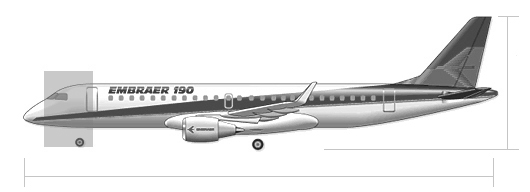
\includegraphics[scale=0.8]{images/ERJ190}
\caption{Posicionamento da LRU}
\label{fig:ERJ190}
\end{figure}


Foi selecionado um objeto sem texturas e com material brilhante como mostrado na
imagem~\ref{fig:LRU} por sofrer mais influ�ncia em varia��o de ilumina��o e ser
�nico na janela de inspe��o em quest�o.

\begin{figure}[h!]
\centering
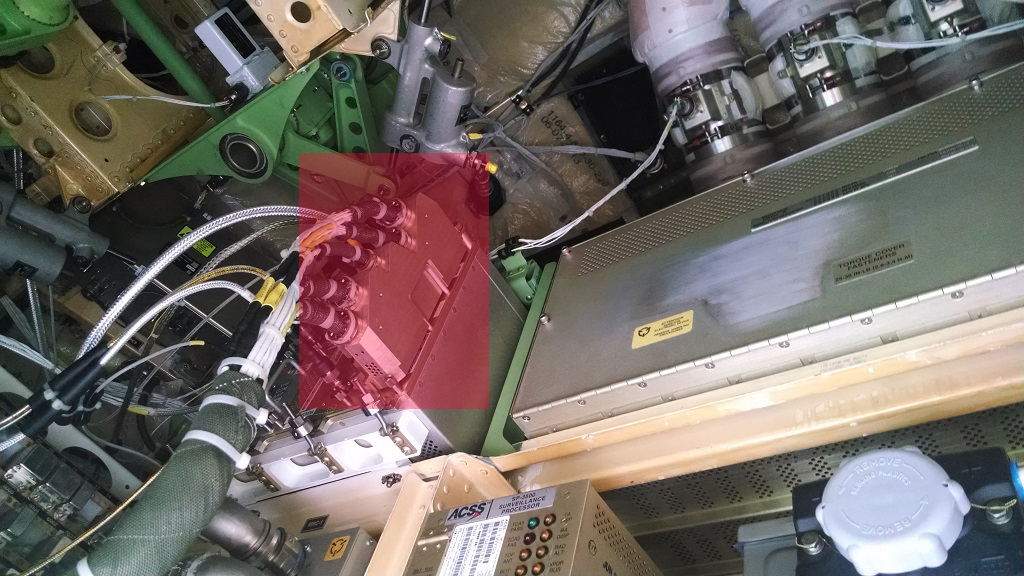
\includegraphics[scale=0.4]{images/LRU}
\caption{Imagem da LRU}
\label{fig:LRU}
\end{figure}

 


 \section{Caso de uso} 

\chapter{Estrutura do texto}
\section{Estrutura}
Este trabalho fundamenta-se em 5 cap�tulos, conforme descritos abaixo:

\begin{itemize}
\item Cap�tulo~\ref{ch:introducao} apresenta a motiva��o do presente trabalho,
levantando as necessidades e limita��es impostas pelo ambiente e o fato de
haverem diversas t�cnicas de reconhecimento de caracter�sticas e a necessidade
de selecionar a adequada para o contexto, bem como descreve o escopo do
trabalho e o contexto em que os testes s�o feitos; 

\item Cap�tulo~\ref{ch:fundamentacaoteorica} tem informa��es suficientes para o entendimento das
an�lises, descrevendo conceitos b�sicos e as t�cnicas de reconhecimento que
foram comparadas;

\item Cap�tulo~\ref{ch:propostao} descreve a metodologia de an�lise adotada bem
como o prot�tipo desenvolvido para a an�lise;

\item Cap�tulo~\ref{ch:analisederesultados} descreve os resultados obtidos comparando-se as
t�cnicas, selecionando qual a t�cnica mais adequada para reconhecimento de
caracter�sticas para o caso de uso descrito;

\item Cap�tulo~\ref{ch:conclusao} conclui o trabalho apresentando como os
objetivos foram atingidos, limita��es da pesquisa e poss�veis
trabalhos futuros.
\end{itemize}


\chapter{Conceitos}
\section{Realidade Aumentada}
A realidade aumentada como citado em \cite{SurveyAR} � uma t�cnica de vis�o
computacional em que valendo-se de artefatos do mundo real tem por objetivo causar sensa��o de imers�o do usu�rio em um ambiente aumentado por artefatos virtuais, ao contr�rio de ambientes puramente virtuais como � comum em aplica��es de realidade virtual.
Idealmente o mundo virtual se torna imersivo o suficiente para que o usu�rio n�o consiga distinguir o real do virtual.
Alguns autores definem AR como tendo a necessidade de utilizar-se interfaces visuais port�teis para que a usabilidade tenha mais coer�ncia com a proposta inicial de garantir uma experi�ncia imersiva.
As imagens s�o obtidas por c�meras e o resultado apresentado em dispositivos como projetores ou 
displays como monitores, tablets ou head-mounted display (HMD). Como mostrado em
\cite{Devices}
\section{Head-Mounted Displays}
� um equipamento utilizado na cabe�a de forma que as duas m�os do usu�rio fiquem livres e tem por objetivo exibir imagens e �udio, sendo uma interface muito utilizada tanto em RV quanto em RA.
Os HMD basicamente s�o dispositivos constitu�dos de duas telas posicionadas frente ao olho do usu�rio.
Com duas telas, a tecnologia pode ser empregada para exibir imagens estereosc�picas apresentando os respectivos pontos de vista de cada olho para cada tela, o que contribui em muito na experi�ncia de imers�o.
Os HMDs funcionam tamb�m como dispositivos de entrada de dados, porque cont�m sensores de rastreamento que medem a posi��o e orienta��o da cabe�a, transmitindo esses dados ao computador.
Existem dois tipos de HMDs: Feed-Through e See-Through
\subsection{Feed-Through}
S�o dispositivos que � um sistema fechado de visualiza��o de imagens, em que o usu�rio consegue enxergar somente o que � mostrado no display, sendo assim o resultado apresentado � sempre a soma da imagem real com informa��es superpostas

\begin{figure}[h!]
\centering
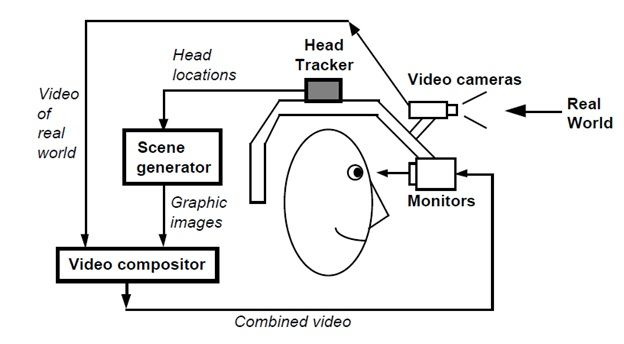
\includegraphics[scale=0.8]{images/feedthrough}
\caption{Arquitetura do Feed-Trough.}
\label{fig:feedthrough}
\end{figure}


\subsection{See-Through}
S�o dispositivos constru�dos com lentes transl�cidas em que o usu�rio enxerga o mundo real e com algum tipo de sistema que sobrepoe na lente as informa��es adicionais

\begin{figure}[h!]
\centering
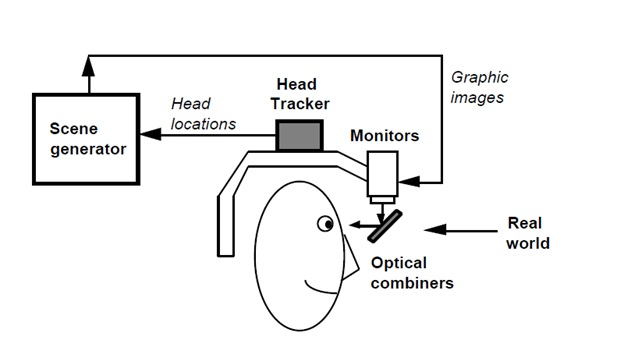
\includegraphics[scale=0.8]{images/seethrough}
\caption{Arquitetura do See-Trough.}
\label{fig:seethrough}
\end{figure}


\subsection{Projetores}
O uso de projetores possibilita uma abordagem de realidade aumentada diferente porque pode ser utilizada para cobrir superf�cies largas, projetando sobre objetos como carros, pessoas, pr�dios, etc�.
Um problema dessa abordagem � que a calibra��o se faz necess�ria em v�rias situa��es.

\subsection{Monitores}
O uso de monitores reduz bastante o custo da aplica��o apesar de ter perda de imers�o por ser um m�todo de visualiza��o indireta, o que implica o usu�rio ficar olhando na dire��o do monitor, entretanto existe a possibilidade de compartilhar os resultados da RA com mais de uma pessoa ao mesmo tempo.

\begin{figure}[h!]
\centering
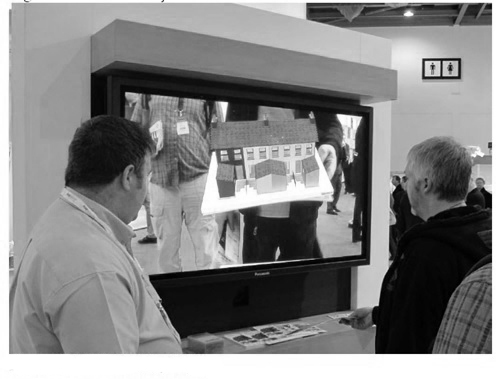
\includegraphics[scale=0.7]{images/monitores}
\caption{Realidade Aumentada com projetores.}
\label{fig:monitores}
\end{figure}

\section{Caracter�sticas Locais}
Caracter�sticas locais s�o padr�es em imagens que diferenciam de seu vizinho imediato, geralmente � caracterizada por mudan�as em propriedades das imagens ou diversas propriedades simultanamente. As propriedades mais comuns s�o intensidade, cor e texturas.

\subsection{Propriedades da Caracter�stica Local ideal}
Algoritmos de reconhecimento baseam-se em compara��o de caracter�sticas recuperadas da cena. A recupera��o e compara��o de pontos tem um custo computacional relevante perto do tempo de execu��o da aplica��o, portanto selecionar o menor n�mero poss�vel de caracter�sticas aumenta o desempenho e diminui o tempo de resposta da aplica��o.
Garantir que estamos selecionando boas caracter�sticas pode ser crucial na efic�cia do reconhecimento.
Segundo \cite{localfeaturedetector} , boas caracter�sticas devem ter as
seguintes propriedades:

\begin{itemize}
	\item \textbf{Repetibilidade}: Dadas duas imagens do mesmo objeto ou cena,
	tomadas em condi��es ou pontos de vista diferentes, uma porcentagem alta de caracter�sticas deve ser reconhecidas se estiverem vis�veis.
	\item \textbf{Distin��o}: Os padr�es reconhecidos t�m de ser poss�veis de serem
	distinguidos entre si para facilitar o casamento.
	\item \textbf{Localidade}: As caracter�sticas devem ser locais para reduzir a
	probabilidade de oclus�o.
	\item \textbf{Quantidade}: O n�mero de pontos detectados tem que ser o
	suficiente para que mesmo objetos pequenos tenham minimamente caracter�sticas que possam ser localizados e para que o 
	objeto possa sofrer oclus�o e ainda assim seja reconhecido.
	\item \textbf{Exatid�o}: As caracter�sticas detectadas tem que ser localizadas
	com o m�ximo de exatid�o poss�vel com respeito tanto referente � posi��o quanto
	� escala.
	\item \textbf{Efici�ncia}:De prefer�ncia  a detec��o deve ser o mais r�pido
	poss�vel.
\end{itemize}

\subsection{Features}
Antes de compreender como � feito o reconhecimento e registro de imagens � importante nos perguntar
 como n�s conseguimos reconhecer objetos em uma cena, como conseguimos comparar facilmente objetos em duas 
 imagens distintas. Somos treinados desde cedo a diferenciar formas geom�tricas, perceber escalas diferentes 
 ou mesmo reconhecer o mesmo objeto independente de como est� posicionado na cena buscando padr�es que 
 categorizem e diferenciem o objeto. Instintivamente conseguimos reconhecer boas caracter�sticas e localizar objetos.
Na imagem~\ref{fig:padroes} temos uma imagem de um pr�dio e seis recortes, dos quais
conseguimos facilmente reconhecer com precis�o a de letra E e F, as de letra A,B,C,D
 podemos identificar poss�veis localiza��es mas n�o podemos dizer com certeza onde est�o na imagem.

\begin{figure}[h!]
\centering
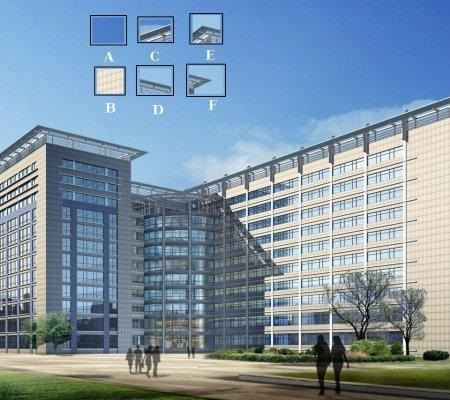
\includegraphics[scale=1.0]{images/features}
\caption{Reconhecimento de padr�es.\cite{understandingfeatures}}
\label{fig:padroes}
\end{figure}
As caracter�sticas E e F s�o o que chamamos de good features pois o n�vel de
certeza � bem alto.

\begin{figure}[h!]
\centering
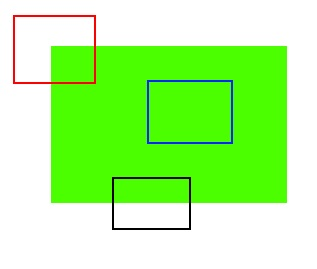
\includegraphics[scale=1.0]{images/featuresregioes}
\caption{Regi�es de reconhecimento de padr�es.\cite{understandingfeatures}}
\label{fig:featuresregioes}
\end{figure}

A Imagem~\ref{fig:featuresregioes} ilustra os tipos de caracter�sticas. A regi�o
azul n�o possibilita diferenciar onde est� na imagem, a regi�o preta pode ser confundida com qualquer uma das regi�es
 ao deslocarmos horizontalmente, a imagem vermelha nos possibilita diferenciar e reconhecer o canto da imagem verde com precis�o milim�trica.
Podemos ent�o concluir que uma caracter�stica � boa para ser utilizada como par�metro de entrada
 para algoritmos de reconhecimento, quanto maior foi o n�vel de certeza da sua localiza��o, 
 o que facilita o \textbf{Feature Detection}.
Para localizar o mesmo objeto em outra imagem � necess�rio identificarmos a regi�o onde se encontra, 
caso contr�rio no exemplo da imagem~\ref{fig:padroes} seria imposs�vel
localizar uma janela espec�fica. Tal descri��o de contexto � chamada de
\textbf{Feature Description}. Uma vez de posse da caracter�stica e do seu
contexto � poss�vel reconhecer o objeto de fato.



\section{Cad�ncia}
� a medida do n�mero de quadros individuais que um determinado dispositivo �ptico ou eletr�nico processa e exibe por unidade de tempo. Em geral a cad�ncia � medida em fps.
Em cinema a cad�ncia de proje��o padr�o desde 1929 foi fixada em 24fps mas no per�odo do cinema mudo a maioria dos filmes eram rodados com cad�ncia entre 16 e 20fps.
Em v�deo, os principais sistemas lidam com cad�ncia entre 25fps(PAL) e 30fps(NTSC).
As aplica��es devem ter cad�ncia toler�vel dependendo de seu uso, segundo \cite{Tang93whydo} para aplica��es interaticas o m�nimo toler�vel � de 5fps enquanto para aplica��es de anima��es fluidas de 30fps.
Sendo a cad�ncia, a freq��ncia entre frames, deve ser contabilizado o tempo de gerar a informa��o e o tempo de dispor a informa��o no dispositivo �ptico.
O tempo de cada frame � calculado por 

\begin{center}
$t_{frame} =  \frac{1}{fps}$
\end{center}

No caso de cad�ncia m�nima de 5fps, temos quadros com tempo menor que 200ms,
portanto as an�lises devem ser balisadas a tempos menores.

\section{Modelo de C�mera}
As c�meras s�o modeladas como c�meras de pequenos orif�cios como mostrada na
imagem~\ref{fig:camera01}.Esse modelo define a proje��o b�sica sobre a qual as
imagens 2D ser�o mapeadas.
Esse modelo � uma simplifica��o optica de uma c�mera real e � utilizado
comumente para descrever a forma��o de imagens na c�mera. O sistema de
coordenadas considerado � a conven��o da m�o direita com centro de coordenadas
de proje��o na origem e a imagem a uma dist�ncia focal f. ref[3]



\begin{figure}[h!]
\centering
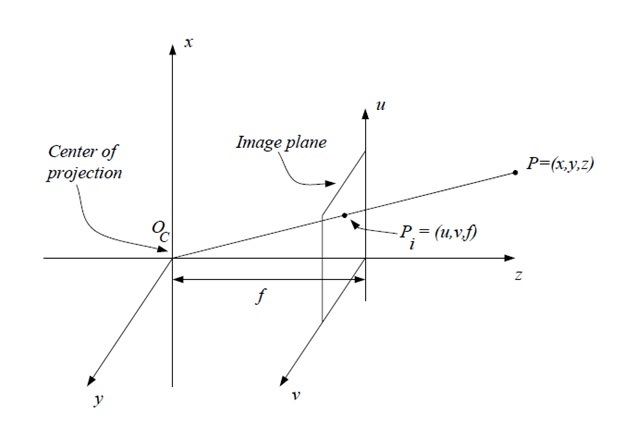
\includegraphics[scale=0.8]{images/camera01}
\caption{Camera no espa�o vetorial.}
\label{fig:camera01}
\end{figure}

\subsection{Calibra��o da C�mera}

Visto que as c�meras atuais adicionam distor��es, se faz necess�rio normalizar as
 imagens antes de utiliz�-las para que os pontos de refer�ncia n�o distor�am tanto na imagem como um todo,
  podendo sofrer efeitos de distor��o nas bordas por exemplo.
Considerando um modelo matem�tico que corrija as distor��es radiais e tangenciais. 
Para corrigir o fator radial, consideramos a seguinte transformada
\begin{figure}[h!]
\centering
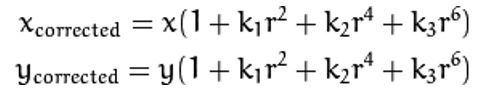
\includegraphics[scale=0.8]{images/camera_eq01}
\caption{Transforma��o de coordenadas}
\label{fig:camera_eq01}
\end{figure}


Em que (x,y) s�o a posi��o do ponto na imagem distorcida,
k1,k2 e k3 s�o constantes a serem descobertas pelo m�todo de calibra��o
r
Para corrigir a distor��o tangencial because image taking lense is not aligned perfectly parallel to the imaging plane.
 So some areas in image may look nearer than expected. It is solved as below:
 
 \begin{figure}[h!]
\centering
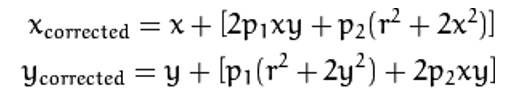
\includegraphics[scale=0.8]{images/camera_eq02}
\caption{Transforma��o de coordenadas quanto � distor��o radial}
\label{fig:camera_eq02}
\end{figure}

Para corrigirmos os dois efeitos e obtermos uma imagem calibrada temos que
resolver a matrix da imagem~\ref{fig:camera_eq03}

 
 \begin{figure}[h!]
\centering
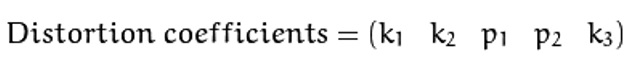
\includegraphics[scale=0.8]{images/camera_eq03}
\caption{Matriz de distor��es}
\label{fig:camera_eq03}
\end{figure}



\section{Reconhecimento}

� a etapa em que padr�es s�o identificados e comparados para posteriormente identificar objetos

 
\begin{figure}[h!]
\centering
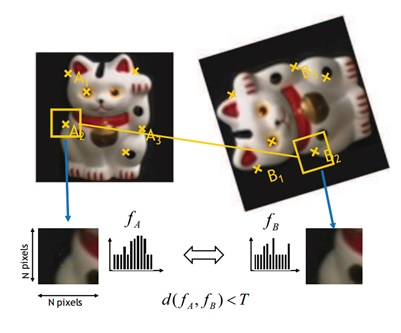
\includegraphics[scale=1.0]{images/reconhecimento}
\caption{Ilustra��o do procedimento de reconhecimento com features locais.}
\label{fig:reconhecimento}
\end{figure}

Pipeline de reconhecimento como ilustrado na imagem~\ref{fig:reconhecimento} :
\begin{itemize}
	\item Encontrar um grupo de keypoints distintos
	\item Definir uma regi�o em torno de cada keypoint 
	\item Extrair e normalizar o conte�do da regi�o
	\item Calcular um descritor para a regi�o normalizada
	\item Encontrar correspond�ncias de descritores.  
\end{itemize}


\section{Caracter�sticas Locais}
Caracter�sticas locais s�o padr�es em imagens que diferenciam padr�es de seu
vizinho imediato, sendo que as mais comuns s�o intensidade, cor e texturas.

\subsection{Caracter�sticas}
Antes de compreender como � feito o reconhecimento e registro de imagens � importante nos perguntar
 como n�s conseguimos reconhecer objetos em uma cena, como conseguimos comparar facilmente objetos em duas 
 imagens distintas. Somos treinados desde cedo a diferenciar formas geom�tricas, perceber escalas diferentes 
 ou mesmo reconhecer o mesmo objeto independente de como est� posicionado na cena buscando padr�es que 
 categorizem e diferenciem o objeto. Instintivamente conseguimos reconhecer boas caracter�sticas e localizar objetos.
Na Figura~\ref{fig:padroes} temos uma Figura de um pr�dio e seis recortes, dos quais
conseguimos facilmente reconhecer com precis�o a de letra E e F, as de letra A,B,C,D
 podemos identificar poss�veis localiza��es mas n�o podemos dizer com certeza onde est�o na Figura.

\begin{figure}[H]
\centering
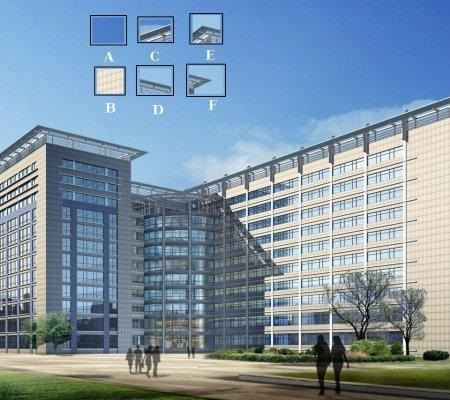
\includegraphics[scale=1.0]{images/features}
\caption{Reconhecimento de padr�es. Fonte \cite{understandingfeatures}}
\label{fig:padroes}
\end{figure}
As caracter�sticas E e F s�o o que consideramos boas caracter�sticas, pois o
n�vel de certeza � bem alto.

\begin{figure}[H]
\centering
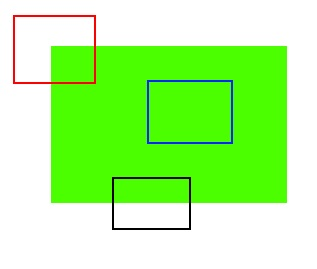
\includegraphics[scale=1.0]{images/featuresregioes}
\caption{Regi�es de reconhecimento de padr�es. Fonte
\cite{understandingfeatures}}
\label{fig:featuresregioes}
\end{figure}

A Imagem~\ref{fig:featuresregioes} ilustra tipos de caracter�sticas. A regi�o
azul n�o possibilita diferenciar onde est� na Figura, a regi�o preta pode ser confundida com qualquer uma das regi�es
 ao deslocarmos horizontalmente, a Figura vermelha nos possibilita diferenciar e reconhecer o canto da Figura verde 
 com precis�o milim�trica.
Podemos ent�o concluir que uma caracter�stica � boa para ser utilizada como par�metro de entrada
 para algoritmos de reconhecimento, quanto maior foi o n�vel de certeza da sua localiza��o, 
 o que facilita o \emph{\textbf{Feature Detection}}.
Para localizar o mesmo objeto em outra Figura � necess�rio identificarmos a regi�o onde se encontra, 
caso contr�rio no exemplo da Figura~\ref{fig:padroes} seria imposs�vel
localizar uma janela espec�fica. Tal descri��o de contexto � chamada de
\emph{\textbf{Feature Description}}. Uma vez de posse da caracter�stica e do seu
contexto � poss�vel reconhecer o objeto de fato.


\subsection{Propriedades da Caracter�stica Local ideal}
Algoritmos de reconhecimento baseam-se em compara��es de caracter�sticas
recuperadas da cena.
A recupera��o e compara��o de pontos tem um custo computacional relevante perto do tempo de execu��o 
da aplica��o, portanto selecionar o menor n�mero poss�vel de caracter�sticas aumenta o desempenho e diminui 
o tempo de resposta da aplica��o.
Garantir que  s�o selecionadas boas caracter�sticas pode ser
crucial na efic�cia do reconhecimento.
Segundo \cite{localfeaturedetector} , boas caracter�sticas devem ter as
seguintes propriedades:

\begin{itemize}
	\item \textbf{Repetibilidade}: Dadas duas imagens do mesmo objeto ou cena,
	tomadas em condi��es ou pontos de vista diferentes, uma porcentagem alta de caracter�sticas deve
	 ser reconhecida se estiverem vis�veis.
	\item \textbf{Distin��o}: Os padr�es reconhecidos t�m de ser poss�veis de serem
	distinguidos entre si para facilitar o casamento.
	\item \textbf{Localidade}: As caracter�sticas devem ser locais para reduzir a
	probabilidade de oclus�o.
	\item \textbf{Quantidade}: O n�mero de pontos detectados tem que ser o
	suficiente para que mesmo objetos pequenos tenham minimamente caracter�sticas que possam ser localizados e para que o 
	objeto possa sofrer oclus�o e ainda assim ser reconhecido.
	\item \textbf{Exatid�o}: As caracter�sticas detectadas tem que ser localizadas
	com o m�ximo de exatid�o poss�vel com respeito tanto referente � posi��o quanto
	� escala.
	\item \textbf{Efici�ncia}:De prefer�ncia  a detec��o deve ser o mais r�pido
	poss�vel.
\end{itemize}



\subsection{Detec��o de caracter�sticas}
O primeiro passo para o reconhecimento de objetos � a detec��o de caracter�sticas.Para que possa ser feita a compara��o da
 imagem referencia com a imagem sentida. A abstra��o de informa��es a ser reconhecida tem que ser suficiente para lidar 
 com escalas diferentes, rota��es entre as imagens, e pequenas distor��es.
Para que o reconhecimento seja eficiente e eficaz s�o necess�rios que uma massa de pontos m�nima seja selecionada e feita
 a correspond�ncia entre as imagens sentidas e refer�ncia.
As caracter�sticas utilizadas s�o em geral cantos, linhas, curvas, padr�es ou regi�es.
O tipo de caracter�stica selecionada � dependente do tipo de imagem provida. Imagens de cenas
 feitas a m�o geralmente s�o compostas de segmentos de retas enquanto imagens de sat�lite s�o geralmente compostas de 
 contornos e regi�es.
Quanto mais invariantes forem as caracter�sticas encontradas, mais robusto e preciso � o processo de compara��o.

\subsection{Correspond�ncia de caracter�sticas}
A fase de correspond�ncia de caracter�sticas � feita tanto selecionando caracter�sticas na imagem refer�ncia e procurando a 
correspondente na imagem sentida ou mesmo selecionando caracter�sticas nas duas imagens independentemente e procurando a 
correspond�ncia entre elas.
Quando a caracter�stica selecionada n�o for do tipo ponto, � importante para cada par de correspond�ncias, pelo menos uma 
ponto ser determinado para que seja utilizado para determinar posteriormente os par�metros de transforma��o. Por exemplo, 
se forem selecionados padr�es como tipo de caracter�stica, o centro do padr�o � considerado o ponto, se for selecionado 
uma regi�o, o centro de massa da regi�o � o ponto de apoio, se linhas forem tomadas como tipo de caracter�stica, devem 
ser tomados intersec��es como ponto de apoio e finalmente se forem selecionadas curvas, os m�ximos locais s�o considerados
 os pontos correspondentes.
 
 \section{Algoritmos de Reconhecimento}
\label{sec:algoritmos}
Existem diversos algoritmos de reconhecimento de caracter�sticas, entretanto
 nesse artigo os testes ser�o restritos aos algoritmos BRISK, FAST, FREAK, GFTT, MSER, ORB,
 STAR, SURF, SIFT.
Este cap�tulo se prop�e a dar uma vis�o geral dos algoritmos, pois o foco do
presente trabalho est� na an�lise comparativa entre os mesmos e n�o em cada um
dos algoritmos, visto exiistir implementa��es conceituadas no OpenCV, framework
utilizado.

%\input{parts/algoritmos/brief}

 \input{parts/algoritmos/fast}
 \input{parts/algoritmos/brisk}

 \input{parts/algoritmos/freak}
 \input{parts/algoritmos/gftt}
 \input{parts/algoritmos/mser}
 \input{parts/algoritmos/orb}
 \input{parts/algoritmos/sift}
 \input{parts/algoritmos/surf}
 \input{parts/algoritmos/star}








\chapter{Metodologia}
\section{Metodologia}
\subsection{Defini��o de par�metros}

Os testes ser�o realizados adicionando vari�veis de forma artificial por meio de transforma��es afins de forma a emular algum comportamento ou situa��o encontrada no ambiente de manuten��o
\begin{itemize}
	\item Varia��o de escala para simular a aproxima��o dentro da janela de
	inspe��o
	\item Varia��o de rota��o para simular a movimenta��o durante a manuten��o
	\item Varia��o de ilumina��o para simular manuten��es feitas em hor�rios do dia
	e ilumina��o diferente como por exemplo ambientes com neve com brilho muito maior
	\item Adi��o de \emph{Blur} para emular ambientes com muita poeira ou
	esfuma�ados
\end{itemize}

A defini��o das faixas de par�metro utilizados foi feita com inspe��o em campo

\section{An�lise de dados}
\label{sec:analisededados}

A an�lise de desempenho de cada t�cnica deve ser balizada por par�metros que garantam que a aplica��o seja vi�vel para o
 contexto citado na Se��o\ref{sec:restricao}. Para tal deve-se considerar os
 par�metros estimados abaixo definidos por inspe��o 

\begin{itemize}
	\item Cad�ncia > 5fps ou seja, tempo < 200ms \cite{Tang93whydo}
	\item Robustez � escala:  0.5 < escala < 1.2
	\item Robustez � rota��o:  0 < rota��o < 30 
	\item Robustez � ilumina��o: -50 < ilumina��o < 50
	\item Robustez � \emph{blur}: \emph{kernelsize} < 4
\end{itemize}

Uma an�lise mais precisa dos par�metros n�o faz parte do escopo desse trabalho
pois envolve pesquisa de campo em situa��es adversas. Portanto tais par�metros
foram escolhidos para validar o m�todo de sele��o das t�cnicas.




\chapter{Prot�tipos}
O escopo de desenvolvimento dessa tese tem por tra�ar um m�todo de escolha do
algoritmo a ser utilizado dependente de aspectos descritos na se��o 2.1 Vari�veis de Contorno, os testes
 ser�o feitos em duas etapas: 
Defini��o de par�metros de contorno e avalia��o dos algoritmos mais conhecidos no contexto aeron�utico

\section{Testes de defini��o de fronteiras de par�metros}

\section{Testes de reconhecimento de padr�es}

Utilizando os par�metros definidos na etapa anterior ser�o rodados todos os algoritmos para avaliar qual se encaixa 
melhor em cada uma das situa��es.
O prot�tipo para testes ser� realizado utilizando o OpenCV por j� disponibilizar os algoritmos mais utilizados para 
o reconhecimento de padr�es e algoritmos de vis�o computacional.
Nesse prot�tipo ser� avaliado a ader�ncia dos algoritmos:Fast, GoodFeaturesToTrack, Mser, Star, Sift, Surf.
Segundo os seguintes crit�rios:\par
\textbf{Velocidade} - para garantir que a aplica��o poder� ser utilizada como
una ferramenta de tempo real � imprescind�vel buscar uma aplica��o que rode naturalmente a 30
 frames por segundo. Tal realidade � facilmente atingida em computadores com v�rios n�cleos 
 como os core i7 mas � importante lembrar que o cen�rio de realidade aumentada para ter um 
 contexto coerente com a proposta de imers�o � composto por dispositivos portateis que via 
 de realidade regra n�o tem poder de processamento t�o alto.\par
\textbf{Qualidade} - ccaracter�sticas detectadas s�o geralmente utilizadas
posteriormente em etapas de rastrio e casamento de padr�o. Para os testes de rastreio
 ser�o adicionadas �s imagens algumas transforma��es afins, como escala, rota��o e ilumina��o
  e ent�o estimar a qualidade das caracter�sticas.\par
\textbf{Ilumina��o e invari�ncia � escala} - Detectores de caracter�sticas tem
que ter a habilidade de reconhecer caracter�sticas independente do tamanho do objeto. A invari�ncia deve ser verdadeira para varia��o de ilumina��o. Varia��es pequenas de ilumina��o e contraste n�o devem afetar o detector significativamente. As c�meras atuais em geral tem controle autom�tico de ganho que ajusta automaticamente a esposi��o evitando sub ou super esposi��o.
\par

Ser�o utilizados as seguintes transforma��es que tem por finalidade avaliar as
varia��es de ambiente
\begin{itemize}
  \item \textbf{Rota��o: }Robustez � rota��o tamb�m � uma caracter�stica
  importante pois nem sempre encontraremos situa��es em que o dispositivo de RA
  sr� posicionado na mesma horienta��o o tempo todo, garantindo uma maior
  autonomia a quem executa a manuten��o
  \item \textbf{Brilho:} A varia��o de brilho pode emular tanto varia��es
  temporais, como dia e noite, mas tamb�m pode emular situa��es de muita
  luminosidade como neve por exemplo
  \item \textbf{Blur: } A robustes a Blur auxilia na resposta do algoritmo
  frente � movimentos bruscos
  \item \textbf{Escala: } A robustez � escala do objeto garante que o mesmo ser�
  reconhecido tanto ao longe quanto em situa��es bem pr�ximas
\end{itemize}


\section{Ambiente}
Os testes tem por objetivo garantir as restri��es descritas na se��o 3. Constraints, portanto � o desempenho e o tempo de reconhecimento s�o uma caracter�stica relevante.
Os resultados obtidos pelos testes descritos nessa tese foram executado em uma m�quina com a seguinte configura��o:

Processador: Core 2-duo 2.2GHz
Mem�ria: 4GB
Placa de V�deo: NVidia GForce 9300M GS

Biblioteca: OpenCV 2.4.10

\subsection{OpenCV}
Distribu�do sob licensa BSD e portanto livre para uso acad�mico e comercial. 
Possui interfaces para C++, C, Python e Java suportando Windows, Linux, Mac OS, iOS 
e Android. OpenCV foi desenvolvido para resultados eficientes e com foco em aplica��es
 de tempo real, podendo tomar vantagem de processamentos paralelos, utilizando-se de OpenCL 
 aproveitando-se da acelera��o de hardware ou mesmo de plataformas heterog�neas. Adotado ao redor
  do mundo em v�rias pesquisas com uma comunidade de  mais de 47 mil pessoas com mais de 9 milh�es
   de downloads. Adotado como plataforma de desenvolvimento para aplica��es de arte interativa a 
   aplica��es de rob�tica avan�ada.
   
 \section{Caso de uso}

Como caso de uso ser� adotado a janela de inspe��o frontal [COLOCAR AQUI UMA 
REFER�NCIA MELHOR] e selecionado uma pe�a. 
A sele��o da pe�a ser� feita de tal forma que contenha informa��es relevantes para estressar 
os limites dos algoritmos de registro, portanto um estudo pr�vio das caracter�sticas dos 
algoritmos para abstrair as caracter�sticas mais relevantes se faz necess�rio. 



ESCREVER as peculiaridades do ambiente para poder decidir qual abordagem vou tomar



\chapter{Resultados}

\cite{performance_evaluation}


Os algoritmos SIFT e SURF apesar de retornarem bons resultados para o contexto,
s�o pagos e portanto ser�o desconsiderados para a abordagem proposta.

Para que sejam respeitados as restri��es citadas na se��o~\ref{sec:restricao} e
para que a aplica��o seja coerente para uso cotidiano no contexto de manuten��o
de aeronaves, a velocidade de reconhecimento � muito importante. Uma an�lise
pr�via dos algoritmos selecionados tem como tempo de resposta por
frame a imagem~\ref{fig:performance6algorithms} que nos mostra claramente que as
t�cnicas MSER e FREAK n�o respondem em tempo �bil para serem considerados tempo
real, portanto ser�o desconsiderados.



\begin{figure}[h!]
\centering
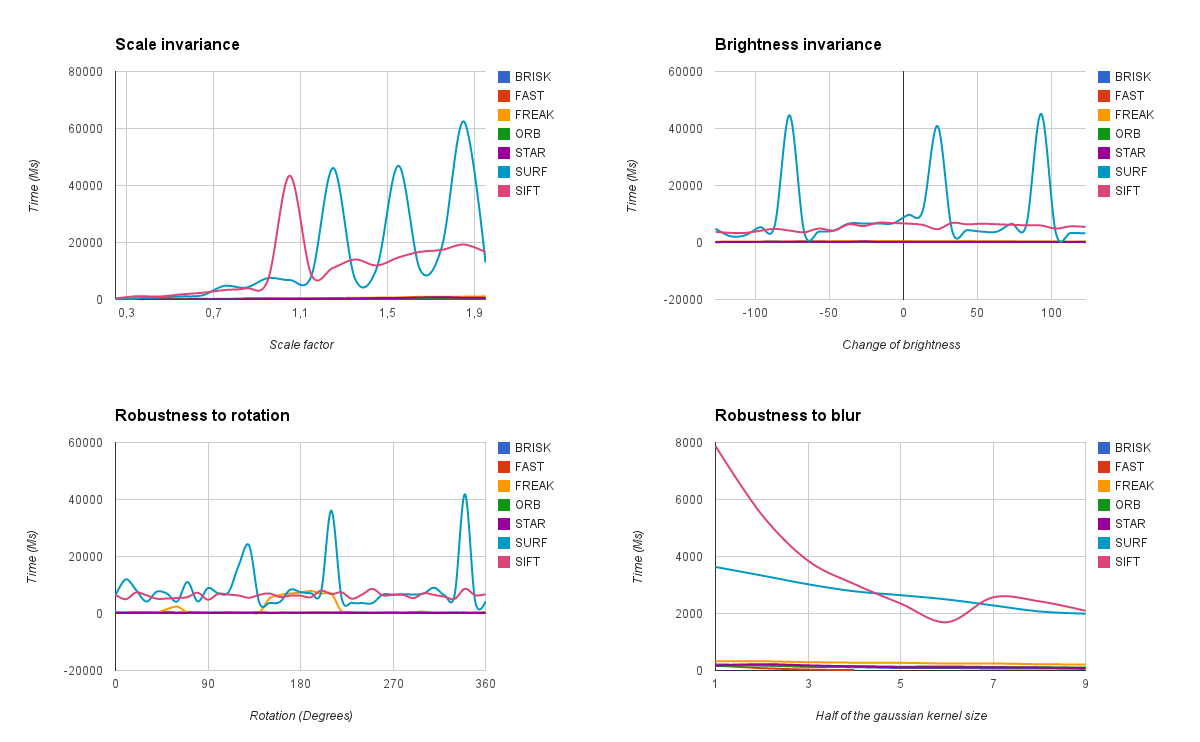
\includegraphics[scale=0.3]{images/time_sift_surf}
\caption{Performance quanto � varia��es de escala, ilumina��o, rota��o e
gaussian blur}
\label{fig:performance6algorithms}
\end{figure}


\begin{figure}[h!]
\centering
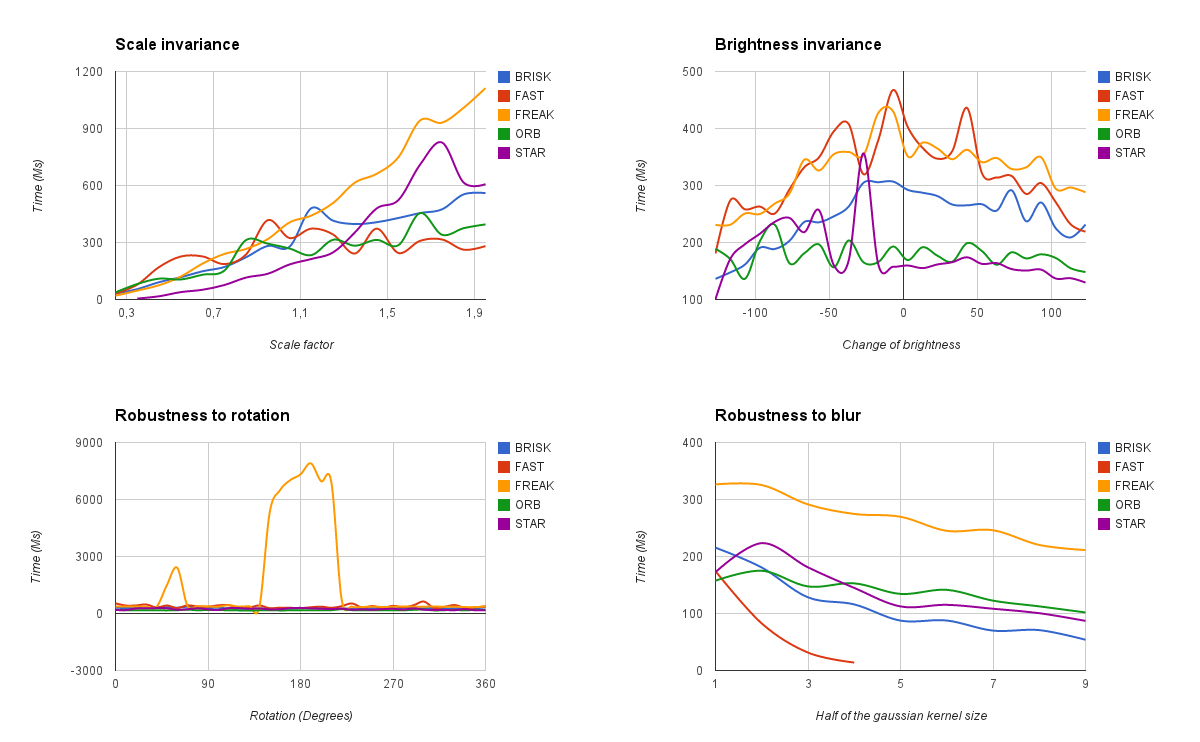
\includegraphics[scale=0.3]{images/time}
\caption{Performance quanto � varia��es de escala, ilumina��o, rota��o e
gaussian blur sem os algoritmos SIFT e SURF}
\label{fig:performance6algorithms}
\end{figure}



\section{Homografia}

Ap�s a etapa de extra��o de caracter�sticas da imagem padr�o e da imagem de
compara��o � importante fazer o casamento de padr�es para que com um n�mero
significativo de caracter�sticas, o objeto seja reconhecido. As imagens
imagem~\ref{fig:blurhomography}, mostram correspond�ncias entre imagens variando
as transforma��es propostas pelo prot�tipo em compara��o com imagens sem as
transforma��es.

\begin{figure}[h!]
\centering
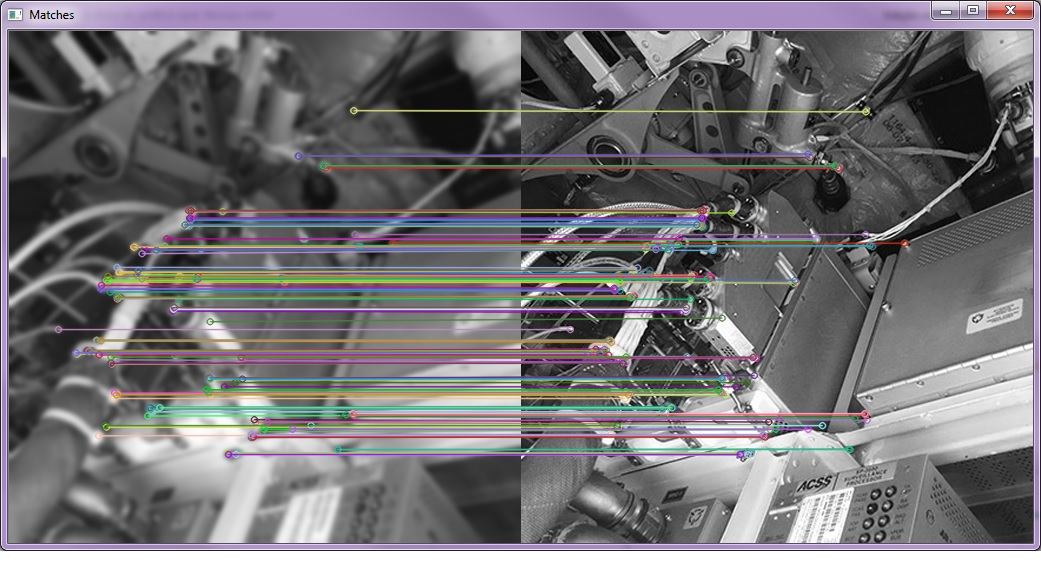
\includegraphics[scale=0.5]{images/ORB-BLUR-HOMOGRAPHY}
\caption{Homografia com varia��o varia��o de Blur.}
\label{fig:blurhomography}
\end{figure}

\begin{figure}[h!]
\centering
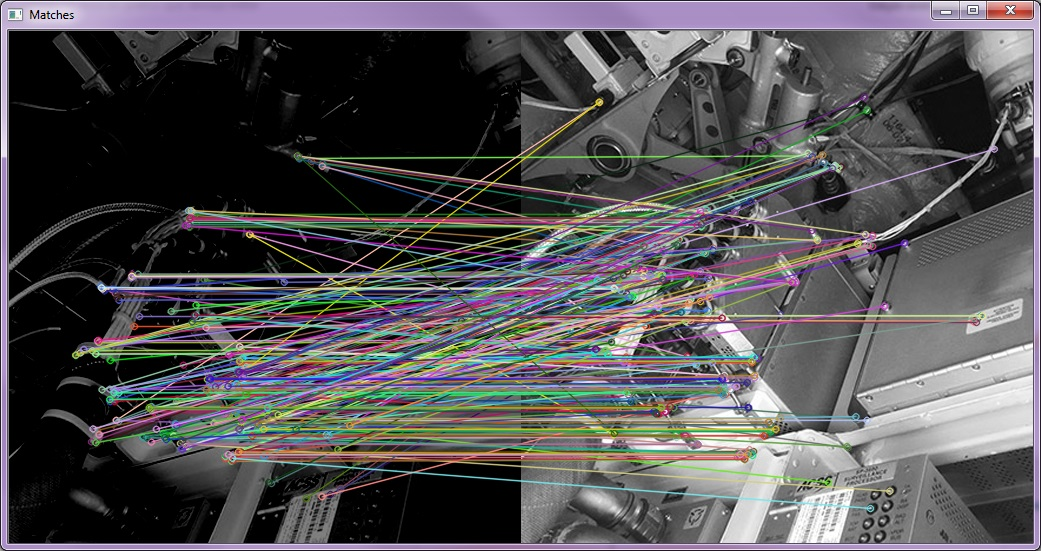
\includegraphics[scale=0.5]{images/ORB-BRIGHT-HOMOGRAPHY}
\caption{Homografia com varia��o varia��o de ilumina��o.}
\label{fig:brighthomography}
\end{figure}




\begin{figure}[h!]
\centering
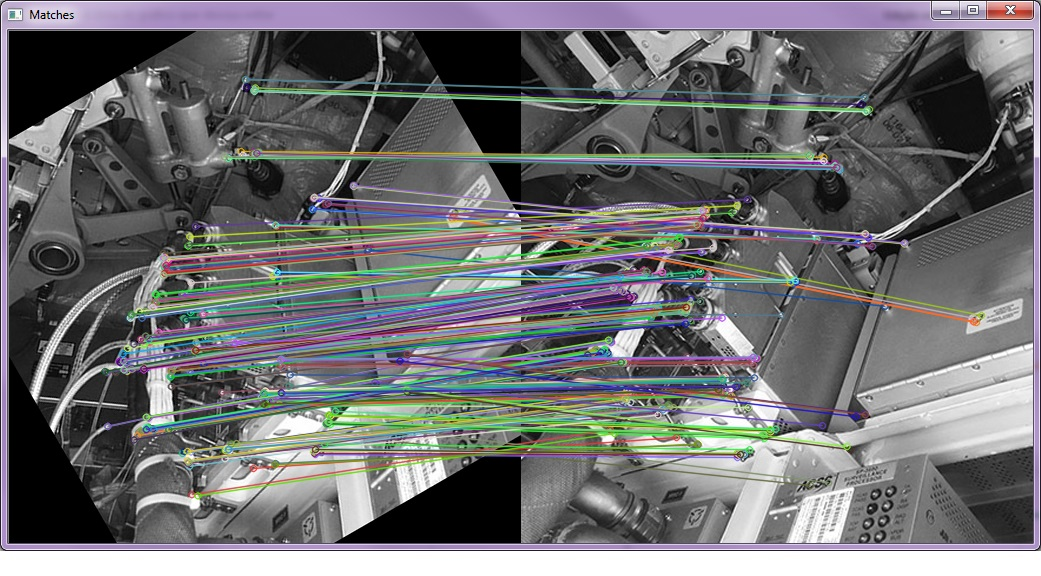
\includegraphics[scale=0.5]{images/ORB-ROTATION-HOMOGRAPHY}
\caption{Homografia com varia��o varia��o de Rota��o.}
\label{fig:rotationhomography}
\end{figure}



\begin{figure}[h!]
\centering
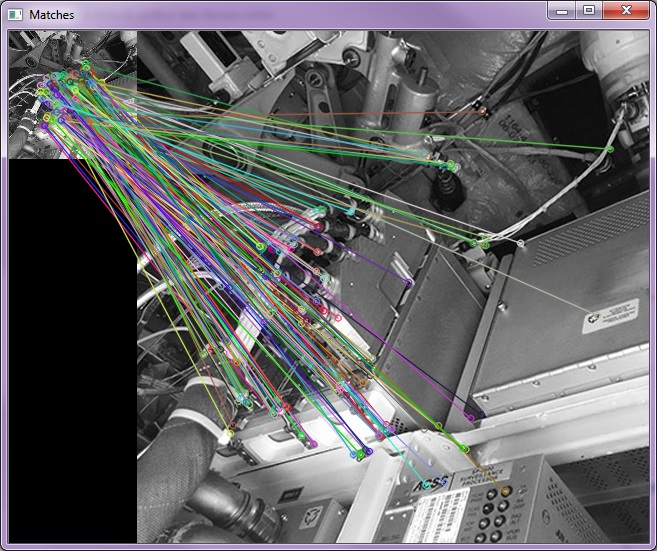
\includegraphics[scale=0.8]{images/ORB-SCALE-HOMOGRAPHY}
\caption{Homografia com varia��o varia��o de Escala.}
\label{fig:scalehomography}
\end{figure}



\cite{ISMAR2012}



\chapter{Conclus�o}
Este trabalho apresentou uma metodologia de compara��o de algoritmos de
reconhecimento de padr�es tendo como caso de uso o contexto aeron�utico, mais
expecificamente no reconhecimento de pe�as do interior da aeronave, objeto de
manuten��o.
Os conceitos b�sicos de Realidade Aumentada e dos algoritmos utlizados foram
apresentados para fornecer meios ao conhecimento dessa tecnologia, que s�o
fundamentais para compreender melhor a proposta do trabalho.
Com o objetivo de tra�ar uma metodologia de decis�o imparcial foram descritos
algumas restri��es impostas � an�lise que posteriormente foram aplicados nos
resultados das simula��es.
Foram feitos testes emulando situa��es de varia��o ambiental pois fazer os
testes em ambientes e situa��es reais demandaria um custo muito elevado, al�m
dos resultados serem semelhantes.
Dessa forma concluiu-se que GFTT Se��o~\ref{sec:gftt}  e ORB Se��o~\ref{sec:orb}
s�o os mais favor�veis para o contexto proposto no trabalho.

\subsection{Atendimento dos objetivos}

\textbf {Avaliar as algoritmos cl�ssicos de reconhecimento}

O trabalho apresentou os algoritmos cl�ssicos na Se��o~\ref{sec:algoritmos},
descrevendo seu funcionamento e realizando testes de desempenho com os mesmos.


\textbf {Selecionar algoritmo mais adequado para o contexto}

Foi feita uma an�lise comparativa entre os algoritmos com as mesmas imagens de
teste e configurando o prot�tipo da mesma maneira, para que a �nica vari�vel no
momento fosse a t�cnica em quest�o.
Levantadas restri��es atrav�s de par�metros emp�ricos definidos por an�lise de
engenharia, com os valores mais prov�veis no contexto.
Para a sele��o das t�cnicas mais adequadas, foram utilizadas as restri��es e
criado nos gr�ficos, janelas de decis�o e gerado uma matriz de decis�o com os
resultados de todos os testes, tanto de qualidade de reconhecimento quanto de
tempo de execu��o.






\chapter{Trabalhos futuros}
\section{Trabalhos Futuros}

A utiliza��o de Realidade Aumentada no campo da manuten��o pode trazer muitos
ganhos no que tange � usabilidade levando ao usu�rio uma quantidade de informa��es que da maneira tradicional por meio inspe��o e consulta em manuais
seria invi�vel.
Este trabalho teve como foco o reconhecimento de padr�es em um cen�rio
aeron�utico espec�fico, como pr�ximos passos temos:
\begin{itemize}

\item Adequar a aplica��o para dispositivos m�veis como tablets, celulares ou
mesmo dispositivos HMD de forma a dar mais flexibilidade ao condutor da
manuten��o;

\item Realizar o casamento de padr�es com v�deos e imagens tempo real utilizando
as t�cnicas identificadas, otimizando a aplica��o para se tornar o mais tempo
real e aceit�vel poss�vel;

\item Adaptar a aplica��o para utilizar processamento paralelo e processamento
em GPU visto os algoritmos serem recursivos e localmente independentes.

\item Analisar por meio de testes em campo com poss�veis usu�rios para abstrair
par�metros de usabilidade como por exemplo determinar que tipo de informa��es
seriam �teis ao usu�rio ou mesmo que tipo de configura��o de dispositivo seria o
mais adequado para uma aplica��o desse porte.
\end{itemize}


% Referencias Bibliograficas
\begin{spacing}{1.0}
\begin{flushleft}
%\bibliographystyle{alpha}%Choose a bibliograhpic style
\bibliography{bibliography}
\end{flushleft}
\end{spacing}


% Apendices
%\appendix
%\chapter{T�picos de �lgebra Linear}
%\input{apendiceA}

% Anexos
%\annex
%\chapter{Exemplo de um Primeiro Anexo}
%\input{anexoA}

% Referencias Bibliograficas



% Glossario
\itaglossary
\printglossary

% Folha de Registro do Documento
% Valores dos campos do formulario
\FRDitadata{24 de dezembro de 1969}
\FRDitadocnro{CTA/ITA - IEC/TM-002/1969}
\FRDitaorgaointerno{Divis�o de Ci�ncia da Computa��o -- ITA/IEC}
\FRDitapalavrasautor{Teses; Estilos; Italus}
\FRDitapalavrasresult{Teses e Disserta��es; Estilos; Usu�rios}
\FRDitaresumo{O reconhecimento de objetos em uma cena para posterior uso em realidade aumentada 
depende de diversas vari�veis, causando a necessidade do uso de t�cnicas 
espec�ficas para cada cen�rio, sendo portanto, um estudo de fronteiras para a melhor escolha 
do algoritmo de reconhecimento, de acordo com a aplica��o em quest�o de grande
valia para o meio acad�mico. 
Esta tese se prop�e a pesquisar, categorizar e tra�ar fronteiras das t�cnicas
conhecidas, tendo como caso de uso a manuten��o de aeronaves feita dentro de
centros fechados, utilizando as t�cnicas BRISK,FAST,FREAK,GFTT,MSER,
 ORB,STAR,SURF,SIFT em uma an�lise aplicada com imagens reais de janelas de
 inspe��o do Embraer ERJ-190 para reconhecimento de objetos e posteriores
 aplica��es em manuten��o.
 Comparando todas as t�cnicas quanto � cad�ncia e � precis�o de reconhecimento
 de caracter�sticas, � poss�vel selecionar GFTT e ORB
 como t�cnicas mais apropriadas ao contexto, por terem seus resultados de
 varia��o de rota��o, escala, briho e \emph{blur} dentro de uma faixa esperada
 para o contexto de manuten��o.
 

}
%  Primeiro Parametro: Nacional ou Internacional -- N/I
%  Segundo parametro: Ostensivo, Reservado, Confidencial ou Secreto -- O/R/C/S
\FRDitaOpcoes{N}{S}
% Cria o formulario
\itaFRD

\end{document}
% Fim do Documento.
